

	%\resizebox{0.98\textwidth}{!}{
	\begin{tabular}{c | c | c | c}
	\hline
	\thead{\footnotesize Class \\ \footnotesize Labels} & \thead{\footnotesize Natural \\ \footnotesize Images} & \thead{\footnotesize Iconic \\ \footnotesize Images} & \thead{\footnotesize Text \\ \footnotesize Descriptions} \\
	\hline 
	\makecell{ \scriptsize Granny Smith \\[-1pt] \scriptsize (Apple)}
	&  \makecell{ \begin{tikzpicture}
			\begin{scope}
				\node {\fbox{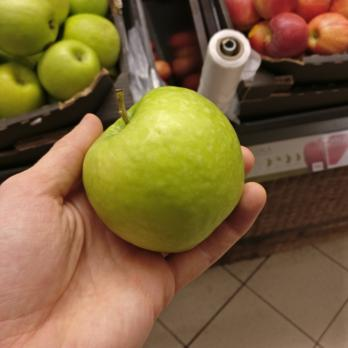
\includegraphics[width=30pt]{Chapter1/pics/Granny-Smith_021.jpg}}};
			\end{scope}
			\begin{scope}[xshift=34pt]
				\node {\fbox{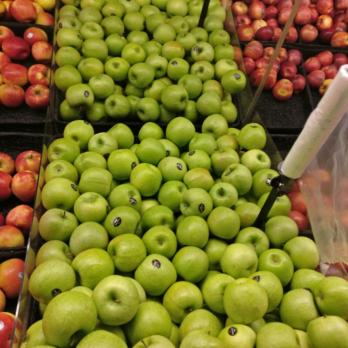
\includegraphics[width=30pt]{Chapter1/pics/Granny-Smith_012.jpg}}};
			\end{scope}
	\end{tikzpicture} }& 
	\makecell{\begin{tikzpicture}
			\begin{scope}
				\node {\fbox{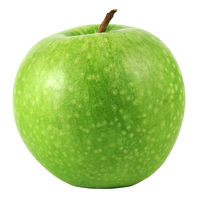
\includegraphics[width=30pt]{Chapter1/pics/Granny-Smith_Iconic.jpg}}};
			\end{scope}
	\end{tikzpicture} } & 
	\begin{scriptsize}
		\makecell{ \textit{“…green apple with white, firm pulp } \\[-1pt]  \textit{and a clear acidity in the flavor.”} } 
	\end{scriptsize}
	\\
	\hline 
	\makecell{ \scriptsize Royal Gala \\[-1pt] \scriptsize (Apple)}
	&  \makecell{ \begin{tikzpicture}
			\begin{scope}
				\node {\fbox{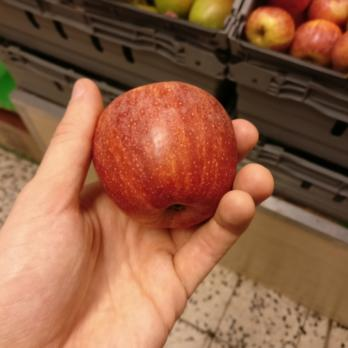
\includegraphics[width=30pt]{Chapter1/pics/Royal-Gala_005.jpg}}};
			\end{scope}
			\begin{scope}[xshift=34pt]
				\node {\fbox{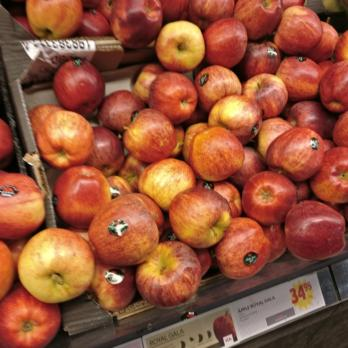
\includegraphics[width=30pt]{Chapter1/pics/Royal-Gala_002.jpg}}};
			\end{scope}
	\end{tikzpicture} }& 
	\makecell{\begin{tikzpicture}
			\begin{scope}
				\node {\fbox{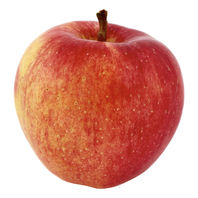
\includegraphics[width=30pt]{Chapter1/pics/Royal-Gala_Iconic.jpg}}};
			\end{scope}
	\end{tikzpicture} } & 
	\begin{scriptsize}
		\makecell{ \textit{“…crispy and very juicy apple,} \\[-1pt] \textit{with yellow-white pulp. The peel} \\[-1pt] \textit{is thin with a red yellow speckled color.”} } 
	\end{scriptsize}
	\\
	\hline
	\makecell{ \scriptsize Tropicana \\[-1pt] \scriptsize Mandarin \\[-1pt] \scriptsize (Juice)}
	&  \makecell{ \begin{tikzpicture}
			\begin{scope}
				\node {\fbox{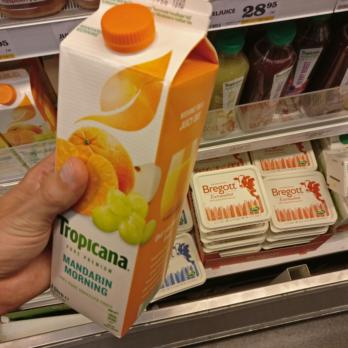
\includegraphics[width=30pt]{Chapter1/pics/Tropicana-Mandarin-Morning_003.jpg}}};
			\end{scope}
			\begin{scope}[xshift=34pt]
				\node {\fbox{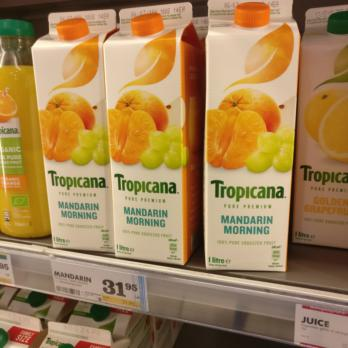
\includegraphics[width=30pt]{Chapter1/pics/Tropicana-Mandarin-Morning_016.jpg}}};
			\end{scope}
	\end{tikzpicture} }& 
	\makecell{\begin{tikzpicture}
			\begin{scope}
				\node {\fbox{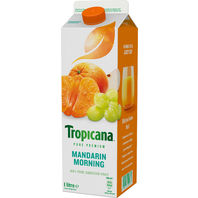
\includegraphics[width=30pt]{Chapter1/pics/Tropicana-Mandarin-Morning_Iconic.jpg}}};
			\end{scope}
	\end{tikzpicture} } & 
	\begin{scriptsize}
		\makecell{ \textit{“…is a ready to drink juice} \\[-1pt]
			\textit{without pulp pressed on orange,} \\[-1pt]
			\textit{ mandarin and grapes. Not from} \\[-1pt]
			\textit{concentrate. Mildly pasteurized.” } }
	\end{scriptsize}
	\\
	\hline
	\makecell{ \scriptsize Yoggi Vanilla \\[-1pt] \scriptsize (Yoghurt)}
	&  \makecell{ \begin{tikzpicture}
			\begin{scope}
				\node {\fbox{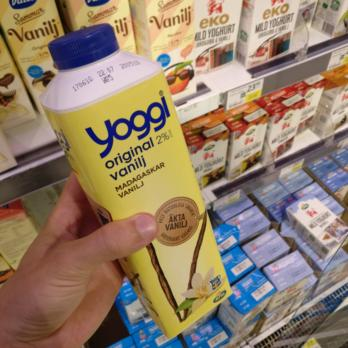
\includegraphics[width=30pt]{Chapter1/pics/Yoggi-Vanilla-Yoghurt_001.jpg}}};
			\end{scope}
			\begin{scope}[xshift=34pt]
				\node {\fbox{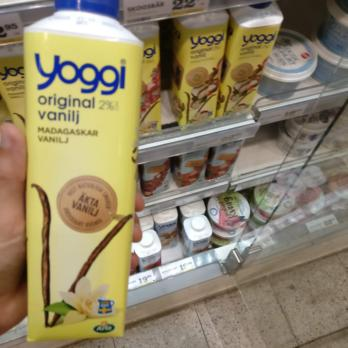
\includegraphics[width=30pt]{Chapter1/pics/Yoggi-Vanilla-Yoghurt_010.jpg}}};
			\end{scope}
	\end{tikzpicture} }& 
	\makecell{\begin{tikzpicture}
			\begin{scope}
				\node {\fbox{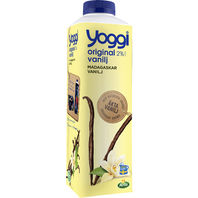
\includegraphics[width=30pt]{Chapter1/pics/Yoggi-Vanilla-Yoghurt_Iconic.jpg}}};
			\end{scope}
	\end{tikzpicture} } & 
	\begin{scriptsize}
		\makecell{ \textit{“...creamy vanilla yoghurt} \\[-1pt]
			\textit{original... added sugar than  } \\[-1pt]
			\textit{regular flavored yoghurt. Great for } \\[-1pt]
			\textit{both breakfast and snacks.”}}
	\end{scriptsize}
	\\
	\hline
\end{tabular}
%}